\documentclass[12pt,oneside]{article} % Uma Coluna e lingua portuguesa
%\usepackage[T1]{fontenc}        % Permite digitar os acentos de forma normal
\usepackage[utf8]{inputenc}
%\usepackage[english]{babel}
\usepackage[portuges,brazil]{babel}
%\usepackage[latin1]{inputenc}
\usepackage[dvips]{graphicx}    % Permite Gráficos
%\usepackage{times}    % Fonte Times
\usepackage{fancyhdr}
\usepackage{array}
\usepackage{multicol}
\usepackage[colorlinks=true,linkcolor=blue,urlcolor=blue]{hyperref}
\usepackage{nomencl}    % glossario
\usepackage{amssymb}
\usepackage{amsmath}
\usepackage[compact]{titlesec}
\usepackage{wrapfig}
\usepackage{color}

%=======================================================================

% Hifenização das palavras desconhecidas pelo LaTeX
%\hyphenation{}
\paperheight    297mm
\paperwidth     210mm
\voffset         -15mm
\headheight      15pt %% tamanho de letra
\headsep         5mm  %% para o início do texto
\oddsidemargin  -3.0mm
\evensidemargin -3.0mm
\textwidth      167.0mm
\topmargin      005.0mm
\textheight     240.0mm
\footskip       10.0mm

\title{SAET 2023 - Maratona de Programação}

\author{Maratona de Programação}
\date{26 de Outubro de 2022}
\usepackage{indentfirst}
\usepackage{subfig}

\parindent=0pt
\setlength{\parskip}{7pt plus 1pt minus 2pt}
\titlespacing{\section}{0pt}{*0}{*0}
\titlespacing{\subsection}{0pt}{*0}{*0}
\titlespacing{\subsubsection}{0pt}{*0}{*0}

\begin{document}

\begin{center}
\textbf{\Huge SAET 2023 - Maratona de Programação} \\
\vspace{0.2cm}
\textit{26 de Outubro de 2022} \\
\vspace{1.0cm}
%\textbf{Sevidor BOCA:} \\
%\texttt{\large http://maratona.c3sl.ufpr.br/boca/} \\
%\vspace{1.0cm}
\begin{figure}[h!]
	\centering
 
\includegraphics[scale=0.95]{capa.png}
\end{figure}
\vspace{1.0cm}
%\textbf{Organizadores:}\\
%{\small Flávio Zavan} \\
%{\small Ricardo Oliveira} \\
\vspace{1.0cm}
\end{center}

\clearpage

\pagestyle{fancy}
\renewcommand{\footrulewidth}{0.7pt}
\renewcommand{\headrulewidth}{0.7pt}
\lhead{SAET 2023 - Maratona de Programação}
%\chead{Maratonas de Programação}
\rhead{26 de Outubro de 2023}
\cfoot{\thepage}

\newpage

\newpage
\section*{A: Alergia} %tle=1
O algoritmo de Manacher[1] encontra, para cada posição $i$ da string, o maior
valor de $j$ tal que $s[i-j..i+j]$ é palíndrome, e o maior valor de $j'$ tal que
$s[i-j'+1..i+j']$ é palíndrome (isto é, o algoritmo consegue determinar, para cada
posição da string, o tamanho da substring palíndrome maximal cujo centro ocorre
naquela posição, tanto a de tamanho ímpar ($j$) quanto a de tamanho par ($j'$)). O algoritmo tem complexidade $O(N)$.

A figura abaixo exemplifica a solução para o exemplo dado no enunciado. O
tamanho obtido pelo algoritmo de Manacher é representado em vermelho:

\begin{center}
    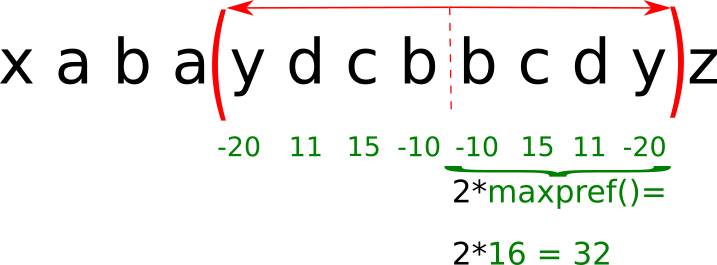
\includegraphics[scale=0.65]{drawkcab/editorial.png}
\end{center}

O próximo passo é determinar o maior valor total possível para cada substring
palindrome maximal. Note que, para substrings de tamanho par, isto é dado por
duas vezes a soma do prefixo de maior soma na segunda metade da substring, e
que, para substrings de tamanho ímpar, é dado por essa soma mais o valor da
letra em seu centro. Na figura exemplificada acima, a resposta é dada por duas vezes a soma do prefixo de maior
soma em $[-10,15,11,-20]$ (que é 16, dado pela soma de $[-10,15,11]$).

Esta soma
pode ser obtida em $O(\lg N)$ através da construção de uma Árvore de
Segmentos adaptada para responder essas consultas, conforme descrito em [2].

Complexidade total: $O(N\lg N)$.

[1] \url{https://cp-algorithms.com/string/manacher.html}

[2] \url{https://www.geeksforgeeks.org/maximum-prefix-sum-given-range/}


\newpage
\section*{B: Jogo} %tle=1
O algoritmo de Manacher[1] encontra, para cada posição $i$ da string, o maior
valor de $j$ tal que $s[i-j..i+j]$ é palíndrome, e o maior valor de $j'$ tal que
$s[i-j'+1..i+j']$ é palíndrome (isto é, o algoritmo consegue determinar, para cada
posição da string, o tamanho da substring palíndrome maximal cujo centro ocorre
naquela posição, tanto a de tamanho ímpar ($j$) quanto a de tamanho par ($j'$)). O algoritmo tem complexidade $O(N)$.

A figura abaixo exemplifica a solução para o exemplo dado no enunciado. O
tamanho obtido pelo algoritmo de Manacher é representado em vermelho:

\begin{center}
    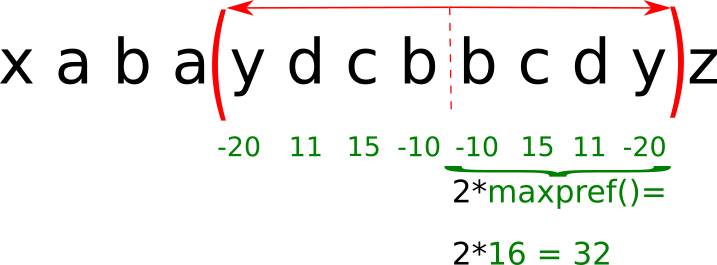
\includegraphics[scale=0.65]{drawkcab/editorial.png}
\end{center}

O próximo passo é determinar o maior valor total possível para cada substring
palindrome maximal. Note que, para substrings de tamanho par, isto é dado por
duas vezes a soma do prefixo de maior soma na segunda metade da substring, e
que, para substrings de tamanho ímpar, é dado por essa soma mais o valor da
letra em seu centro. Na figura exemplificada acima, a resposta é dada por duas vezes a soma do prefixo de maior
soma em $[-10,15,11,-20]$ (que é 16, dado pela soma de $[-10,15,11]$).

Esta soma
pode ser obtida em $O(\lg N)$ através da construção de uma Árvore de
Segmentos adaptada para responder essas consultas, conforme descrito em [2].

Complexidade total: $O(N\lg N)$.

[1] \url{https://cp-algorithms.com/string/manacher.html}

[2] \url{https://www.geeksforgeeks.org/maximum-prefix-sum-given-range/}


\newpage
\section*{C: Vasilha Errada} %tle=1
O algoritmo de Manacher[1] encontra, para cada posição $i$ da string, o maior
valor de $j$ tal que $s[i-j..i+j]$ é palíndrome, e o maior valor de $j'$ tal que
$s[i-j'+1..i+j']$ é palíndrome (isto é, o algoritmo consegue determinar, para cada
posição da string, o tamanho da substring palíndrome maximal cujo centro ocorre
naquela posição, tanto a de tamanho ímpar ($j$) quanto a de tamanho par ($j'$)). O algoritmo tem complexidade $O(N)$.

A figura abaixo exemplifica a solução para o exemplo dado no enunciado. O
tamanho obtido pelo algoritmo de Manacher é representado em vermelho:

\begin{center}
    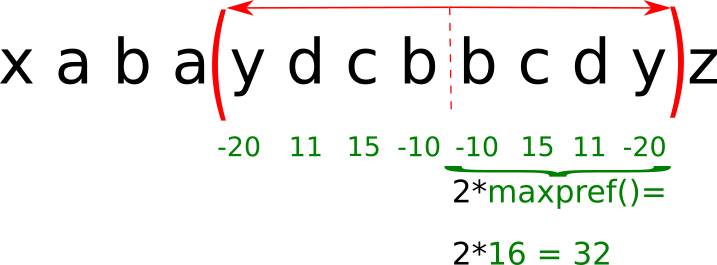
\includegraphics[scale=0.65]{drawkcab/editorial.png}
\end{center}

O próximo passo é determinar o maior valor total possível para cada substring
palindrome maximal. Note que, para substrings de tamanho par, isto é dado por
duas vezes a soma do prefixo de maior soma na segunda metade da substring, e
que, para substrings de tamanho ímpar, é dado por essa soma mais o valor da
letra em seu centro. Na figura exemplificada acima, a resposta é dada por duas vezes a soma do prefixo de maior
soma em $[-10,15,11,-20]$ (que é 16, dado pela soma de $[-10,15,11]$).

Esta soma
pode ser obtida em $O(\lg N)$ através da construção de uma Árvore de
Segmentos adaptada para responder essas consultas, conforme descrito em [2].

Complexidade total: $O(N\lg N)$.

[1] \url{https://cp-algorithms.com/string/manacher.html}

[2] \url{https://www.geeksforgeeks.org/maximum-prefix-sum-given-range/}


\newpage
\section*{D: Drawkcabackward} %tle=1
O algoritmo de Manacher[1] encontra, para cada posição $i$ da string, o maior
valor de $j$ tal que $s[i-j..i+j]$ é palíndrome, e o maior valor de $j'$ tal que
$s[i-j'+1..i+j']$ é palíndrome (isto é, o algoritmo consegue determinar, para cada
posição da string, o tamanho da substring palíndrome maximal cujo centro ocorre
naquela posição, tanto a de tamanho ímpar ($j$) quanto a de tamanho par ($j'$)). O algoritmo tem complexidade $O(N)$.

A figura abaixo exemplifica a solução para o exemplo dado no enunciado. O
tamanho obtido pelo algoritmo de Manacher é representado em vermelho:

\begin{center}
    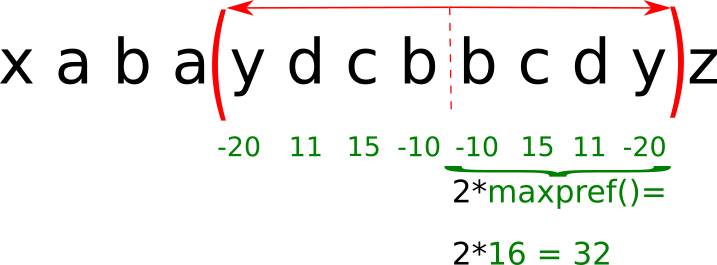
\includegraphics[scale=0.65]{drawkcab/editorial.png}
\end{center}

O próximo passo é determinar o maior valor total possível para cada substring
palindrome maximal. Note que, para substrings de tamanho par, isto é dado por
duas vezes a soma do prefixo de maior soma na segunda metade da substring, e
que, para substrings de tamanho ímpar, é dado por essa soma mais o valor da
letra em seu centro. Na figura exemplificada acima, a resposta é dada por duas vezes a soma do prefixo de maior
soma em $[-10,15,11,-20]$ (que é 16, dado pela soma de $[-10,15,11]$).

Esta soma
pode ser obtida em $O(\lg N)$ através da construção de uma Árvore de
Segmentos adaptada para responder essas consultas, conforme descrito em [2].

Complexidade total: $O(N\lg N)$.

[1] \url{https://cp-algorithms.com/string/manacher.html}

[2] \url{https://www.geeksforgeeks.org/maximum-prefix-sum-given-range/}


\newpage
\section*{E: Empilha Copos} %tle=1
O algoritmo de Manacher[1] encontra, para cada posição $i$ da string, o maior
valor de $j$ tal que $s[i-j..i+j]$ é palíndrome, e o maior valor de $j'$ tal que
$s[i-j'+1..i+j']$ é palíndrome (isto é, o algoritmo consegue determinar, para cada
posição da string, o tamanho da substring palíndrome maximal cujo centro ocorre
naquela posição, tanto a de tamanho ímpar ($j$) quanto a de tamanho par ($j'$)). O algoritmo tem complexidade $O(N)$.

A figura abaixo exemplifica a solução para o exemplo dado no enunciado. O
tamanho obtido pelo algoritmo de Manacher é representado em vermelho:

\begin{center}
    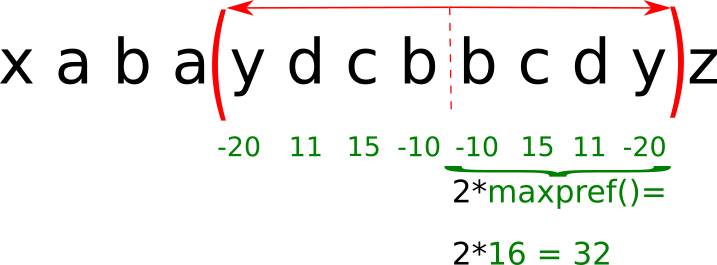
\includegraphics[scale=0.65]{drawkcab/editorial.png}
\end{center}

O próximo passo é determinar o maior valor total possível para cada substring
palindrome maximal. Note que, para substrings de tamanho par, isto é dado por
duas vezes a soma do prefixo de maior soma na segunda metade da substring, e
que, para substrings de tamanho ímpar, é dado por essa soma mais o valor da
letra em seu centro. Na figura exemplificada acima, a resposta é dada por duas vezes a soma do prefixo de maior
soma em $[-10,15,11,-20]$ (que é 16, dado pela soma de $[-10,15,11]$).

Esta soma
pode ser obtida em $O(\lg N)$ através da construção de uma Árvore de
Segmentos adaptada para responder essas consultas, conforme descrito em [2].

Complexidade total: $O(N\lg N)$.

[1] \url{https://cp-algorithms.com/string/manacher.html}

[2] \url{https://www.geeksforgeeks.org/maximum-prefix-sum-given-range/}


\newpage
\section*{F: Falco} %tle=1
O algoritmo de Manacher[1] encontra, para cada posição $i$ da string, o maior
valor de $j$ tal que $s[i-j..i+j]$ é palíndrome, e o maior valor de $j'$ tal que
$s[i-j'+1..i+j']$ é palíndrome (isto é, o algoritmo consegue determinar, para cada
posição da string, o tamanho da substring palíndrome maximal cujo centro ocorre
naquela posição, tanto a de tamanho ímpar ($j$) quanto a de tamanho par ($j'$)). O algoritmo tem complexidade $O(N)$.

A figura abaixo exemplifica a solução para o exemplo dado no enunciado. O
tamanho obtido pelo algoritmo de Manacher é representado em vermelho:

\begin{center}
    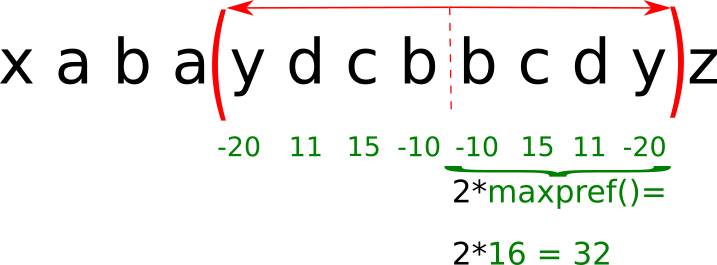
\includegraphics[scale=0.65]{drawkcab/editorial.png}
\end{center}

O próximo passo é determinar o maior valor total possível para cada substring
palindrome maximal. Note que, para substrings de tamanho par, isto é dado por
duas vezes a soma do prefixo de maior soma na segunda metade da substring, e
que, para substrings de tamanho ímpar, é dado por essa soma mais o valor da
letra em seu centro. Na figura exemplificada acima, a resposta é dada por duas vezes a soma do prefixo de maior
soma em $[-10,15,11,-20]$ (que é 16, dado pela soma de $[-10,15,11]$).

Esta soma
pode ser obtida em $O(\lg N)$ através da construção de uma Árvore de
Segmentos adaptada para responder essas consultas, conforme descrito em [2].

Complexidade total: $O(N\lg N)$.

[1] \url{https://cp-algorithms.com/string/manacher.html}

[2] \url{https://www.geeksforgeeks.org/maximum-prefix-sum-given-range/}


\newpage
\section*{G: Gafe} %tle=1
O algoritmo de Manacher[1] encontra, para cada posição $i$ da string, o maior
valor de $j$ tal que $s[i-j..i+j]$ é palíndrome, e o maior valor de $j'$ tal que
$s[i-j'+1..i+j']$ é palíndrome (isto é, o algoritmo consegue determinar, para cada
posição da string, o tamanho da substring palíndrome maximal cujo centro ocorre
naquela posição, tanto a de tamanho ímpar ($j$) quanto a de tamanho par ($j'$)). O algoritmo tem complexidade $O(N)$.

A figura abaixo exemplifica a solução para o exemplo dado no enunciado. O
tamanho obtido pelo algoritmo de Manacher é representado em vermelho:

\begin{center}
    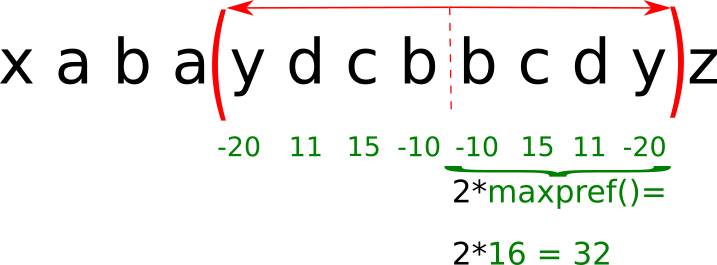
\includegraphics[scale=0.65]{drawkcab/editorial.png}
\end{center}

O próximo passo é determinar o maior valor total possível para cada substring
palindrome maximal. Note que, para substrings de tamanho par, isto é dado por
duas vezes a soma do prefixo de maior soma na segunda metade da substring, e
que, para substrings de tamanho ímpar, é dado por essa soma mais o valor da
letra em seu centro. Na figura exemplificada acima, a resposta é dada por duas vezes a soma do prefixo de maior
soma em $[-10,15,11,-20]$ (que é 16, dado pela soma de $[-10,15,11]$).

Esta soma
pode ser obtida em $O(\lg N)$ através da construção de uma Árvore de
Segmentos adaptada para responder essas consultas, conforme descrito em [2].

Complexidade total: $O(N\lg N)$.

[1] \url{https://cp-algorithms.com/string/manacher.html}

[2] \url{https://www.geeksforgeeks.org/maximum-prefix-sum-given-range/}


\newpage
\section*{H: Raid} %tle=1
O algoritmo de Manacher[1] encontra, para cada posição $i$ da string, o maior
valor de $j$ tal que $s[i-j..i+j]$ é palíndrome, e o maior valor de $j'$ tal que
$s[i-j'+1..i+j']$ é palíndrome (isto é, o algoritmo consegue determinar, para cada
posição da string, o tamanho da substring palíndrome maximal cujo centro ocorre
naquela posição, tanto a de tamanho ímpar ($j$) quanto a de tamanho par ($j'$)). O algoritmo tem complexidade $O(N)$.

A figura abaixo exemplifica a solução para o exemplo dado no enunciado. O
tamanho obtido pelo algoritmo de Manacher é representado em vermelho:

\begin{center}
    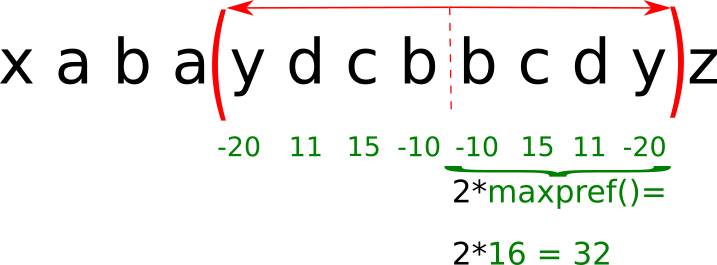
\includegraphics[scale=0.65]{drawkcab/editorial.png}
\end{center}

O próximo passo é determinar o maior valor total possível para cada substring
palindrome maximal. Note que, para substrings de tamanho par, isto é dado por
duas vezes a soma do prefixo de maior soma na segunda metade da substring, e
que, para substrings de tamanho ímpar, é dado por essa soma mais o valor da
letra em seu centro. Na figura exemplificada acima, a resposta é dada por duas vezes a soma do prefixo de maior
soma em $[-10,15,11,-20]$ (que é 16, dado pela soma de $[-10,15,11]$).

Esta soma
pode ser obtida em $O(\lg N)$ através da construção de uma Árvore de
Segmentos adaptada para responder essas consultas, conforme descrito em [2].

Complexidade total: $O(N\lg N)$.

[1] \url{https://cp-algorithms.com/string/manacher.html}

[2] \url{https://www.geeksforgeeks.org/maximum-prefix-sum-given-range/}


\newpage
\section*{I: Lista} %tle=1
O algoritmo de Manacher[1] encontra, para cada posição $i$ da string, o maior
valor de $j$ tal que $s[i-j..i+j]$ é palíndrome, e o maior valor de $j'$ tal que
$s[i-j'+1..i+j']$ é palíndrome (isto é, o algoritmo consegue determinar, para cada
posição da string, o tamanho da substring palíndrome maximal cujo centro ocorre
naquela posição, tanto a de tamanho ímpar ($j$) quanto a de tamanho par ($j'$)). O algoritmo tem complexidade $O(N)$.

A figura abaixo exemplifica a solução para o exemplo dado no enunciado. O
tamanho obtido pelo algoritmo de Manacher é representado em vermelho:

\begin{center}
    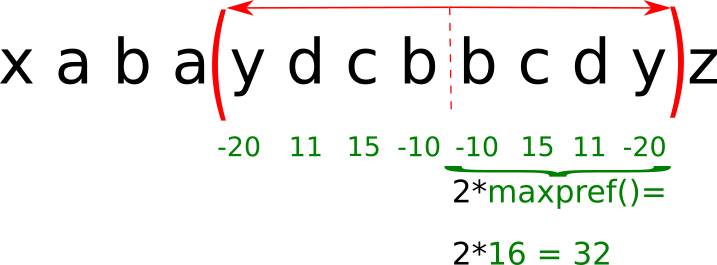
\includegraphics[scale=0.65]{drawkcab/editorial.png}
\end{center}

O próximo passo é determinar o maior valor total possível para cada substring
palindrome maximal. Note que, para substrings de tamanho par, isto é dado por
duas vezes a soma do prefixo de maior soma na segunda metade da substring, e
que, para substrings de tamanho ímpar, é dado por essa soma mais o valor da
letra em seu centro. Na figura exemplificada acima, a resposta é dada por duas vezes a soma do prefixo de maior
soma em $[-10,15,11,-20]$ (que é 16, dado pela soma de $[-10,15,11]$).

Esta soma
pode ser obtida em $O(\lg N)$ através da construção de uma Árvore de
Segmentos adaptada para responder essas consultas, conforme descrito em [2].

Complexidade total: $O(N\lg N)$.

[1] \url{https://cp-algorithms.com/string/manacher.html}

[2] \url{https://www.geeksforgeeks.org/maximum-prefix-sum-given-range/}


\newpage
\section*{J: Meuzamigo} %tle=1
O algoritmo de Manacher[1] encontra, para cada posição $i$ da string, o maior
valor de $j$ tal que $s[i-j..i+j]$ é palíndrome, e o maior valor de $j'$ tal que
$s[i-j'+1..i+j']$ é palíndrome (isto é, o algoritmo consegue determinar, para cada
posição da string, o tamanho da substring palíndrome maximal cujo centro ocorre
naquela posição, tanto a de tamanho ímpar ($j$) quanto a de tamanho par ($j'$)). O algoritmo tem complexidade $O(N)$.

A figura abaixo exemplifica a solução para o exemplo dado no enunciado. O
tamanho obtido pelo algoritmo de Manacher é representado em vermelho:

\begin{center}
    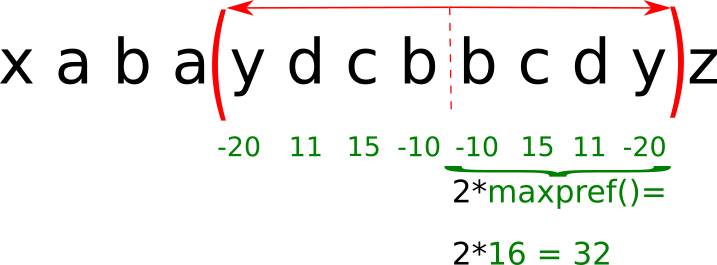
\includegraphics[scale=0.65]{drawkcab/editorial.png}
\end{center}

O próximo passo é determinar o maior valor total possível para cada substring
palindrome maximal. Note que, para substrings de tamanho par, isto é dado por
duas vezes a soma do prefixo de maior soma na segunda metade da substring, e
que, para substrings de tamanho ímpar, é dado por essa soma mais o valor da
letra em seu centro. Na figura exemplificada acima, a resposta é dada por duas vezes a soma do prefixo de maior
soma em $[-10,15,11,-20]$ (que é 16, dado pela soma de $[-10,15,11]$).

Esta soma
pode ser obtida em $O(\lg N)$ através da construção de uma Árvore de
Segmentos adaptada para responder essas consultas, conforme descrito em [2].

Complexidade total: $O(N\lg N)$.

[1] \url{https://cp-algorithms.com/string/manacher.html}

[2] \url{https://www.geeksforgeeks.org/maximum-prefix-sum-given-range/}


\newpage
\section*{K: Tiras} %tle=1
O algoritmo de Manacher[1] encontra, para cada posição $i$ da string, o maior
valor de $j$ tal que $s[i-j..i+j]$ é palíndrome, e o maior valor de $j'$ tal que
$s[i-j'+1..i+j']$ é palíndrome (isto é, o algoritmo consegue determinar, para cada
posição da string, o tamanho da substring palíndrome maximal cujo centro ocorre
naquela posição, tanto a de tamanho ímpar ($j$) quanto a de tamanho par ($j'$)). O algoritmo tem complexidade $O(N)$.

A figura abaixo exemplifica a solução para o exemplo dado no enunciado. O
tamanho obtido pelo algoritmo de Manacher é representado em vermelho:

\begin{center}
    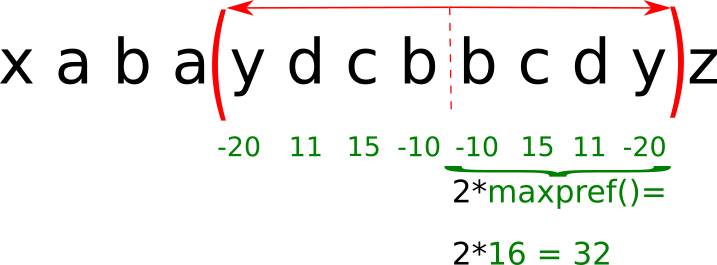
\includegraphics[scale=0.65]{drawkcab/editorial.png}
\end{center}

O próximo passo é determinar o maior valor total possível para cada substring
palindrome maximal. Note que, para substrings de tamanho par, isto é dado por
duas vezes a soma do prefixo de maior soma na segunda metade da substring, e
que, para substrings de tamanho ímpar, é dado por essa soma mais o valor da
letra em seu centro. Na figura exemplificada acima, a resposta é dada por duas vezes a soma do prefixo de maior
soma em $[-10,15,11,-20]$ (que é 16, dado pela soma de $[-10,15,11]$).

Esta soma
pode ser obtida em $O(\lg N)$ através da construção de uma Árvore de
Segmentos adaptada para responder essas consultas, conforme descrito em [2].

Complexidade total: $O(N\lg N)$.

[1] \url{https://cp-algorithms.com/string/manacher.html}

[2] \url{https://www.geeksforgeeks.org/maximum-prefix-sum-given-range/}


\end{document}
